\chapter{Introducción general}

En este capítulo se presenta el marco general del trabajo. Se detallan las motivaciones que llevaron a Trenes Argentinos a solicitar su desarrollo, y se realiza una revisión del estado del arte en cuanto a los productos comerciales disponibles. Se describe la propuesta inicial y las razones por las que posteriormente se decidió descartarla, y se exponen el alcance y los objetivos de la propuesta final.

\label{cap:IntroGeneral}

\section{Motivación}

La empresa Trenes Argentinos \cite{web:sofse} adquirió en 2013 un total de 705 unidades eléctricas múltiples (EMU) a la empresa china CRRC Qingdao Sifang \cite{web:sifang} \cite{licitacion1}. Estos vehículos prestan servicios en las líneas Mitre, Sarmiento y Roca desde 2014 \cite{emu:roca} \cite{emu:mitre-sarmiento}.

% TODO: la licitacion1 es para las lineas Sarmiento y Mitre. Falta la de Roca.
% TODO: esta bien citar wikipedia?

\begin{figure}[htbp]
	\centering
	\includegraphics[width=.5\textwidth]{./Figures/1082px-Línea_Mitre_Retiro.jpg}
	\caption[Unidad eléctrica múltiple (EMU)]{Una unidad eléctrica múltiple (EMU) en la estación Retiro de la línea Mitre, en Buenos Aires.\footnotemark}
	\label{fig:emu}
\end{figure}
\footnotetext{Fotografía por Casa Rosada (Argentina Presidencia de la Nación), CC BY-SA 2.0, \url{https://commons.wikimedia.org/w/index.php?curid=39117175}}

Los distintos subsistemas electrónicos presentes en una EMU (control de frenos, control de tracción, control de puertas, paneles de información al pasajero, etc.) están interconectados formando una red de datos. Mediante esta red, los componentes comparten datos de diagnóstico y reciben órdenes de control a distancia. La red interna que se utiliza en las EMU es una implementación del estándar TCN (Train Communication Network, IEC 61375-1 \cite{iec61375-1}).

Actualmente, Trenes Argentinos carece del conocimiento y las herramientas necesarias para interactuar con la red TCN en las EMU, de forma tal de poder capturar la información disponible, o agregar dispositivos de desarrollo propio.
Además, no dispone de un sistema de monitoreo a distancia que permita observar en tiempo real el estado de cada uno de los componentes de una formación ferroviaria.
Tampoco cuenta con un sistema de almacenamiento histórico del estado de los componentes, de forma tal de poder hacer pericia en caso de un accidente.

Estas limitaciones se vuelven más evidentes con frecuencia. Un ejemplo común es cuando una formación queda varada en un punto alejado de una estación, obligando a los técnicos a trasladarse personalmente para resolver el problema.
También es común la quema de fusibles, un inconveniente difícil de diagnosticar sin el monitoreo de variables como la tensión de línea.
Otro desafío adicional es la falta de control sobre las variables del sistema de aire acondicionado, lo que dificulta garantizar el confort y la seguridad de los pasajeros.


\section{Estado del arte}

La norma IEC 61375-1 es la fuente de información principal acerca del estándar TCN. Lamentablemente no hay mucha información adicional de libre acceso acerca del estándar, como artículos y notas de aplicación. Entre las publicaciones que citan a la norma tal vez las más relevantes son \textit{Design and implementation of MVB protocol analyzer} \cite{mvb-pub-1} (escrita en idioma chino) y \textit{An MVB signal capturer based on microcontrollers for metro train on-line health monitoring system} \cite{mvb-pub-2}, siendo ambas demasiado cortas como para aportar información realmente útil.

La mayoría de los equipos desarrollados hasta la fecha que funcionan de acuerdo al estándar TCN se basa en dos ASICs\footnote{Application-specific integrated circuit.} diferentes: el circuito MVBCS1 \cite{mvbcs1}, producido originalmente por la compañía ABB, aunque hoy en día es comercializado por Siemens, y el MVBC02C \cite{mvbc02c}, producido por Bombardier. Debido a su naturaleza, estos circuitos presentan características rígidas que no son apropiadas para satisfacer la amplia gama de posibilidades con respecto al tipo de nodos conectados a la red TCN \cite{mvb-pub-3}.

Otra publicación de interés es \textit{A Novel SoC Architecture for a MVB Slave Node} \cite{mvb-pub-3}, donde se describe el diseño de una arquitectura SoC\footnote{System on a chip.} compatible con el estándar TCN, basado en una FPGA\footnote{Field-programmable gate array.}.

Es posible encontrar en el mercado soluciones más intergadas, que podrían proporcionar una solución parcial a los problemas que afronta Trenes Argentinos. A continuación se presentan algunos de estos dispositivos, así como sus características principales.

\subsection{Yacer -- MVB-Analyzer}

El analizador de protocolo \textit{MVB-Analyzer} de la empresa Yacer \cite{yacer} proporciona una interfaz MVB, dos interfaces Ethernet y dos interfaces de expansión para recopilar y recibir tramas MVB y WTB, entre otras, y enviarlas a una computadora a través de una interfaz Ethernet. El producto incluye un software que permite analizar los datos del bus MVB y realizar simulaciones para encontrar la resolución de problemas y evaluar el funcionamiento del bus MVB.

\begin{figure}[htbp]
	\centering
	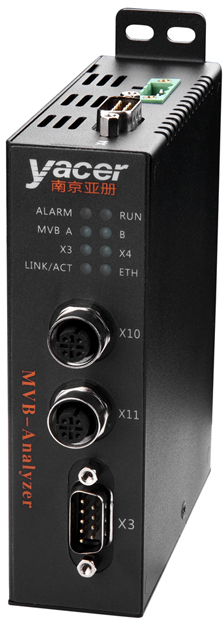
\includegraphics[height=20\baselineskip]{./Figures/yacer.jpg}
	\caption[Yacer -- MVB-Analyzer]{El analizador de protocolo \textit{MVB-Analyzer} de la empresa Yacer.}
\end{figure}

\subsection{AMiT Transportation -- WTB and MVB Analyzers}

Los analizadores del bus WTB y MVB de la empresa AMiT Transportation \cite{amit} son dispositivos de bus pasivos que monitorean el tráfico en la red y lo pasan al bus Ethernet en tramas UDP. Se conecta una PC al bus Ethernet con un programa para recibir y evaluar las tramas UDP.

El analizador solo monitorea el bus, y es "invisible" para otros dispositivos. Se monitorean todas las tramas WTB o MVB en el bus, que son transmitidas por el bus Ethernet a la PC. El producto incluye un complemento para el programa de código abierto Wireshark \cite{wireshark}, que permite analizar las tramas capturadas.

\begin{figure}[htbp]
	\centering
	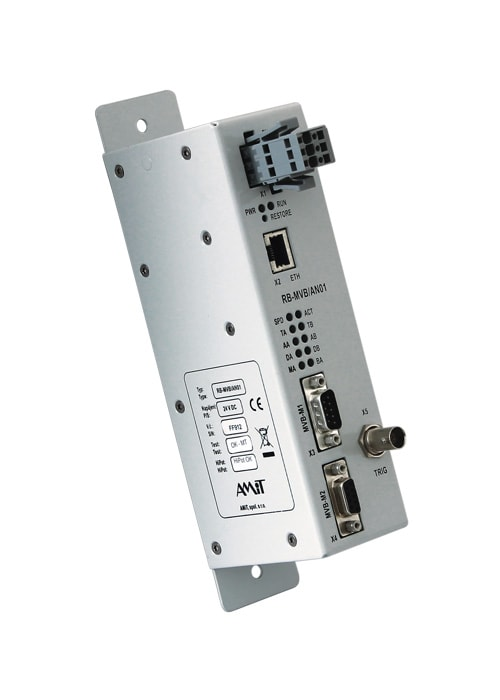
\includegraphics[height=20\baselineskip]{./Figures/amit.jpg}
	\caption[AMiT Transportation -- WTB and MVB Analyzers]{El analizador de bus MVB de la empresa AMiT Transportation.}
\end{figure}


\subsection{Duagon -- D442 MVB Diagnostic System}

El sistema de diagnóstico MVB de la empresa Duagon \cite{duagon} está diseñado para depurar dispositivos y redes MVB. El sistema se conecta a una PC común, y puede funcionar en dos modos de operación:

\begin{itemize}
\item En el modo \emph{monitor}, el sistema permite investigar dispositivos MVB en el bus, leer y escribir la base de datos MVB, y escanear los puertos de los dispositivos, entre otras cosas.
\item En el modo \emph{servidor}, el sistema permite ejecutar aplicaciones programadas por el usuario. Se incluye una biblioteca de programación MVB con todas las funciones en el sistema de diagnóstico para controlar una red MVB completa.
\end{itemize}

\begin{figure}[htbp]
	\centering
	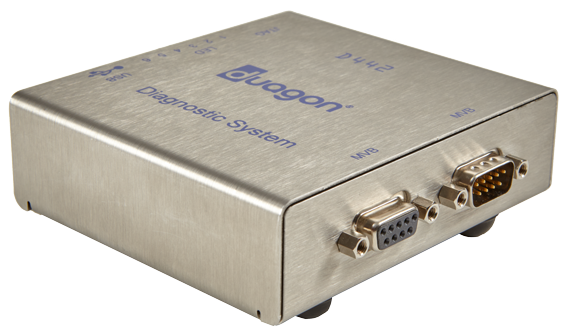
\includegraphics[width=0.5\textwidth]{./Figures/duagon.png}
	\caption[Duagon -- D442 MVB Diagnostic System]{El sistema de diagnóstico MVB de la empresa Duagon}
\end{figure}


\section{Propuesta inicial}

% En este contexto, Trenes Argentinos y el Grupo de Investigación en Calidad y Seguridad de las Aplicaciones Ferroviarias (GICSAFe) \cite{web:gicsafe} arman un grupo de trabajo para encontrar una solución.


\section{Alcance y objetivos}
